\subsection{Vehicular ad hoc Networks}

\acrshort{VANET} - is a network that combines \acrshort{V2V} (Vehicle-to-vehicle) and \acrshort{V2I} (Vehicle-to-infrastructure) communication.\par
% 
\begin{figure}[ht]
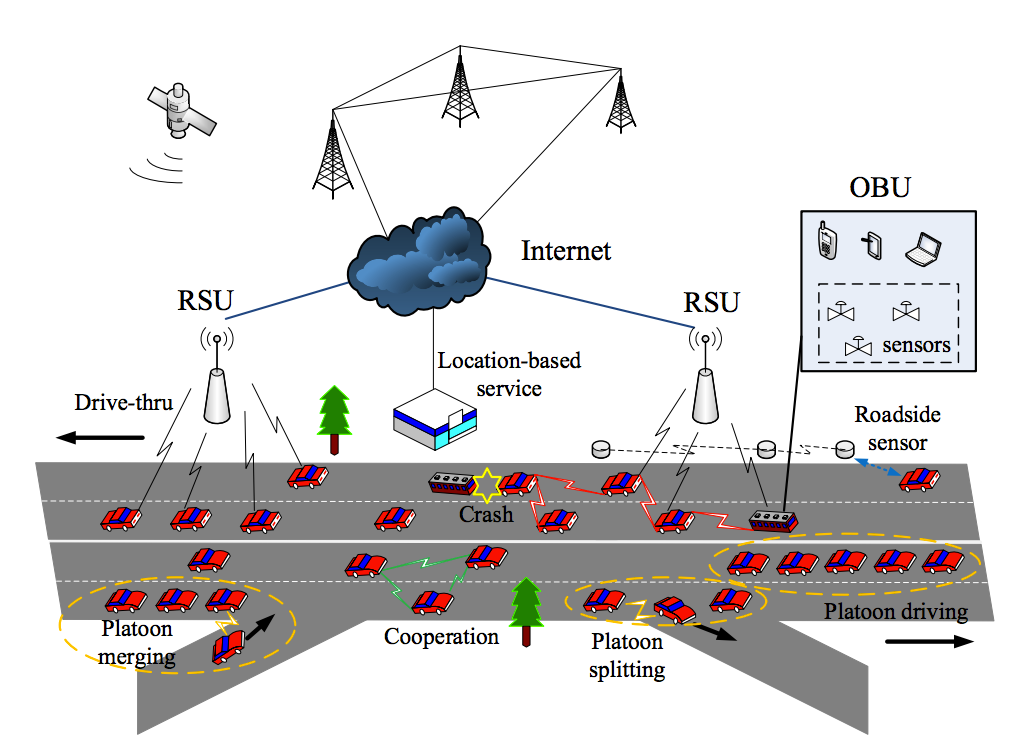
\includegraphics[width=\textwidth]{VANET}
\caption{\acrshort{VANET} formation. In this scenario, all the vehicles are equipped with an \acrshort{OBU} (shown in detail on the right), and can thus communicate with the \acrshort{RSU} and each other. Figure taken from \cite{Jia2016ASystems}.}
% \centering
\label{fig:VANETformation}
\end{figure}
% 
It is large and complex network where vehicles exchange data between each other and any other infrastructure on the road. Traffic participant might receive data, that will prevent accident from happening, relayed from multiple interconnected nodes. Generally \acrshort{VANET}s introduce:

\begin{itemize}[noitemsep,nolistsep]
    \item Safer and more efficient roads
    \item Logistics, transport and service business improvement
    \item Controlled congestion, more comfortable travelling.
\end{itemize}

In Figure \ref{fig:VANETformation} we can see the general architecture of \acrshort{VANET}. One main disadvantage that slows down VANET development that it is dependant on expensive road infrastructure\footnotemark.\par
% 
\footnotetext{\url{http://wifinotes.com/mobile-communication-technologies/what-is-vanet.html}, accessed on 19/04/2017}
% 
\acrshort{VANET} is based on latest mobile communication technologies. Following chapters will discuss present and upcoming technologies that make up the VANET - namely \acrshort{V2V} and \acrshort{V2I}, as these are most relevant for platooning use.
